\subsection{Ejercicios}
\begin{exercise}[1]
Se desea estudiar el envío de paquetes de 128 bytes en una red de conmutación de paquetes con encaminamiento fijo. El enlace entre nodos tiene una capacidad de 64kbps.\\
\textbf{1.} ¿Qué modelo de sistema de colas se puede aplicar?.\\
Se trata de un sistema M/M/1\\
\textbf{2.} ¿Cuál es el número medio de paquetes servidos por segundo?\\
\[\mu=8\sfrac{KB}{s}\frac{1Paquete}{128Bytes}=62.5\sfrac{Paquetes}{s}\]
\textbf{3.} ¿Cuál es el número medio de paquetes por segundo que un nodo puede aceptar para que el tiempo medio de espera en el buffer sea igual a 10 segundos?\\
\begin{gather*}
W_q=\frac{\rho}{\mu(1-\rho)}=10s\\
\rho=\frac{A_c}{c}=A_o=\frac{\lambda}{\mu}\to \lambda=\rho \mu\\
W_q=\frac{\rho}{\mu(1-\rho)}\to\rho=\frac{W_q \mu}{1+W_q\mu}=0.9984\\
\lambda=62.4\sfrac{Paquetes}{s}
\end{gather*}
\textbf{4.} ¿Cuánta memoria en media se estará ocupando en el nodo?\\
\[\text{Memoria}=L_q128=128\frac{\rho^2}{1-\rho}=79.744kB=637.9kb\]
\[L_q=623 \text{ Paquetes en cola de media}\]
\end{exercise}
\begin{exercise}[2]
Un conmutador monoproceso de servicio 16 horas al día FCFS(First Come First Serve) a un conjunto de usuarios. El patrón de llegadas programadas es poissonianode media 20 programas/día y la distribución de tiempo de CPU  de cada programa es exponendial de media 30 minutos.\\
\textbf{1.} ¿Cuál será el factor de utilización de la CPU?\\
Se trata de un M/M/1 con lo cual $\rho=A_o$.\\
\[\rho=\frac{\lambda}{\mu}=\frac{20*30}{60*16}=0.625=62.5\%\]
\textbf{2.} Se reciben quejas de los usuarios, ¿a qué puede ser debido?\\
\[W_q=\frac{\rho}{\mu(1-\rho)}=50\text{ minutos}\]
Se está casi el doble de tiempo en cola que dentro del servidor. Este será el motivo de queja mayoritario.\\
\textbf{3.} Se decide colocar en paralelo tantas CPUs como sean necesarias para garantizar que el tiempo medio de espera en cola sea inferior o como máximo de 10 minutos. ¿Cuántos deben colocarse?\\
\begin{gather*}
A_c=A_o=0.625\\
\rho=\frac{A_c}{c}=\frac{A_o}{c}\\
W_q=E(s)\frac{C(A_o,c)}{c(1-\rho)}
\end{gather*}
Hallaremos la respuesta por prueba y error:
\begin{center}
\begin{tabular}{c|c|c|c}
CPU & $\rho$ & $C(A_o,c)$ & $W_q$ \\\hline
2 & 0.3125 & 0.15 & 3.27 min\\
3 & 0.208 & 0.03 & 0.38 min
\end{tabular}
\end{center}
Como se puede ver en la tabla con solamente añadir un segundo servidor se puede conseguir el objetivo de estar menos de 10 minutos en la cola.\\
\textbf{4.} ¿Es conveniente instalar 2 CPUs que se repartan los usuarios de forma que cada una atienda por separado a la mitad de las peticiones recibidas?\\
Aquí se puede ver que vuelve a ser un sistema M/M/1 con $\lambda=10\sfrac{programas}{dia}$.
\begin{gather*}
\rho=A_o=\frac{\lambda}{\mu}=\frac{30*10}{60*16}=0.3125\\
W_q=E(s)\frac{\rho}{1-\rho}=13.63 \text{ minutos de espera de media}
\end{gather*}
Como se puede ver 13.63\textgreater \textgreater 3.27. Con esto se demuestra que los sistemas de cola única son mucho más eficientes.
\end{exercise}
\begin{exercise}[3]
Los usuarios de una población infinita demandan poisonianamente con tasa 0.1 demandas/segundo un recurso sin cola de espera, con c servidores idénticos. El servicio demandado es exponencial de media E(s). Se desea garantizar que el tiempo de respuesta no sea superior a 10 segundos para al menos el 80\% de los usuarios, y se quiere perder menos del 15\% de los usuarios.\\
\textbf{1.} Calcular E(s) para cumplir con los valores requeridos.\\
\begin{gather*}
p(t<10s)=1-e^{-10\mu}=0.8 \to \mu=0.16\sfrac{\text{demandas}}{\text{segundo}}\\
E(s)=\frac{1}{\mu}=6.25\sfrac{\text{s}}{\text{demanda}}
\end{gather*}
\textbf{2.} ¿Cuántos servidores es necesario colocar?\\
Con $A_o=\sfrac{\lambda}{\mu}=0.625E$ y $P_B<15\%$ miramos en la gráfica de Erlang B y obtenemos que el número de servidores c ha de ser mayor o igual a 2.\\
\textbf{3.} ¿Cuántos servidores están desocupados en media?\\
$L=L_s=A_c=A_o(1-P_B)=0.53125$ usuarios de media en el sistema con lo cual hay 1.46875 servidores libres de media en el sistema.
\end{exercise}
\begin{exercise}[4]
Se dispone de una red de terminales de comunicaciones que acceden a un controlador central según un esquema ALOHA ranurado con parámetro k=5. La capacidad del canal es de 56 Kbps y cada terminal manda en media 1 paquete de 1000 bits de duración cada 100 segundos. La distancia de cada uno de los terminales al controlador es de 3km y el tiempo que tarda en generar un paquete ACK es de 10 mseg.\\
\textbf{1.} ¿Cuántos terminales pueden compartir el canal si el rendimiento del sistema es la mitad del máximo posible?\\
\begin{gather*}
S=I=\frac{S_{max}}{2}=0.18\\
I=\frac{Na_o}{C}\\
C=56Kbps=56*1024=57344bbps\\
a_o=\frac{1000bits}{100s}=10bps\\
N=1032terminales
\end{gather*}
\textbf{2.} ¿Cuantos intentos hay que hacer en media para transmitir con éxito un paquete?\\
Para obtener el valor de G haremos una tabla donde por prueba y error intentaremos aproximarnos al valor de S=0.18.
\begin{gather*}
S=Ge^{-G}\\
\frac{G}{S}=\frac{0.2255}{0.18}=1.25 intentos
\end{gather*}
\begin{center}
\begin{tabular}{c | c}
G & S \\\hline
0.1 & 0.009\\
0.2 & 0.1637\\
0.3 & 0.22\\
0.25 & 0.19\\
0.2255 & 0.18\\
\end{tabular}
\end{center}
Como se puede ver tanto 0.2 como 0.3 se aproximan bastante y serian suficientemente buenos para un examen.\\
\textbf{3.} ¿Cuántos servidores están desocupados en media?\\
\begin{gather*}
D=1.5+a+(\frac{G}{S}-1)(1.5+2a+w+\frac{1+k}{2})=2.86\\
t_a=\frac{d}{c}=\frac{3*10^3}{3*10^8}=10^{-5}seg\\
m=\frac{1000}{56*1024}=0.0174\sfrac{seg}{paq}\\
a=\frac{t}{m}=57.34*10^{-3}\\
w=\frac{t_{ACK}}{m}=1.5734
\end{gather*}
\end{exercise}
\begin{exercise}[5]
La red telefónica de la figura tiene una probabilidad de pérdidas en las secciones finales del 1\% y una probabilidad de desbordamiento en las secciones directas del 10\% .
\begin{figure}[H]
\centering
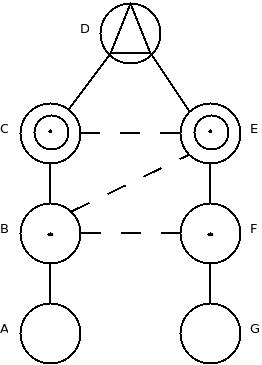
\includegraphics[width=0.5\textwidth]{Imagen/ejercicio5tema1.jpg}
\label{}
\end{figure}
La matriz de tráfico (simétrica) en Erlangs es la siguiente:
\begin{center}
\begin{tabular}{| c | c | c | c | c | c | c | c |}
\hline
   & A & B & C & D & E & F & G \\\hline
 A & - & 10 & 15 & 5 & 2 & 1 & 1 \\\hline
 B &   & - & 50 & 15 & 6 & 3 & 2 \\\hline
 C &   &   & - & 80 & 30 & 10 & 5 \\\hline
 D &   &   &   & - & 90 & 15 & 5 \\\hline
 E &   &   &   &   & - & 60 & 18 \\\hline
 F &   &   &   &   &   & - & 12 \\\hline
\end{tabular}
\end{center}
Se pide:\\
\textbf{1.} Indicar los caminos que comunican los nodos E y A.\\
\begin{center}
\begin{tabular}{c c c c}
E$\to$A & EBA  		& A$\to$E 	& ABE 	\\
 		& EDCBA		&			& ABCE	\\
 		& 			&			& ABCDE	\\
\end{tabular}
\end{center}
\textbf{2.} Calcular el tráfico ofrecido y cursado en la sección directa C$\to$E.\\
\begin{gather*}
TO_{C\to E}=TO_{CEpropio}+TO_{BEdesb}+TO_{BFdesb}+TO_{CF}+TO_{CG}=\\
30+0.8+0.7+10+5=46.5E\\
TO_{BE}=TO_{BEpropio}+TO_{AE}=8E\\
TO_{BEdesb}=TO_{BE}P_d=TO_{BE}0.1=0.8E\\
TO_{BF}=TO_{BFpropio}+TO_{BG}+TO_{AF}+TO_{AG}=7E\\
TO_{BFdesb}=TO_{BF}P_d=TO_{BF}0.1=0.7E\\
TC_{C\to E}=TO_{C\to E}(1-P_D)=41.85E
\end{gather*}
\textbf{3.} Considerando solo el tráfico saliente de A y sabiendo que la probabilidad de que la duración de la llamada sea superior a 5 minutos es de 0.08205, ¿cuál es la duración media de la llamada?\\
Se trata de un sistema con bloqueo M/M/c/c con $A_{oA}=34E=\frac{\lambda}{\mu}$.
\begin{gather*}
P(W>5min)=\int_{5}^{\infty}\mu e^{-\mu t}dt=-e^{-\mu t}\Big|_{5}^{\infty}=0.08205\\
\mu=0.5\sfrac{llamadas}{minuto}\to E(s)=2\sfrac{minutos}{llamada}
\end{gather*}
\textbf{4.} ¿Cuántos intentos de llamada se hacen en la hora cargada(HC)?\\
\begin{gather*}
A_{oA}=34E=\frac{\lambda}{\mu}\\
\mu=0.5\sfrac{llamadas}{minuto}\\
\lambda=34*0.5=17\sfrac{llamadas}{minuto}\\
\lambda_{HC}=17*60=1020\sfrac{llamadas}{hora}
\end{gather*}
\textbf{5.} Los registradores de la central A analizan las primeras cifras y encaminan las llamadas, pudiéndose modelar como un sistema M/M/c. Si el tiempo de ocupación de los registradores por cada llamada es de 6 segundos, ¿cuántos son necesarios para que la probabilidad de esperar más de 1 segundo sea de 0.008?\\
\begin{gather*}
E(s')=6\sfrac{segundos}{llamada}\to A'_o=\frac{\lambda}{\mu '}=1.7E\\
P(W_q>1s)=0.008=C(c,A'_o)e^-c\mu 'T(1-\rho)
\end{gather*}
Este apartado habrá que hacerlo por prueba y error hasta hallar el número de servidores necesarios para cumplir con las especificaciones. Se puede ver estas pruebas en la tabla:\\
\begin{center}
\begin{tabular}{c | c | c | c}
$C(c,A'_o)$ & c & $\rho$ & $P(W_q>1)$ \\\hline
0.7  & 2 & 0.85  & 0.6672 \\
0.1  & 4 & 0.425 & 0.0692 \\
0.008 & 6 & 0.283 & 0.00402
\end{tabular}
\end{center} 
De la tabla se puede observar que el número mínimo de registradores ha de ser 6.\\
\textbf{6.} ¿Cuál es el tiempo medio de espera en los registradores?\\
\[W_q=\frac{E(s)\rho}{1-\rho}=2.3682segundos\]
\end{exercise}
\begin{exercise}[6]
En un territorio de un país en vías de desarrollo, se ha decidido crear una nueva red telefónica digital. Para su planificación se han considerado los siguientes datos:
\begin{itemize}
\item Tras agrupar geográficamente los diferentes núcleos en entidades de población, resultando 83, se han obtenido 70 entidades  con 20000 habitantes, 10 con 60000, 2 con 1000000 y 1 (la capital) con 2000000
\item Se considera un grado inicial de penetración del servicio del 30\% (30 teléfonos por cada 100 habitantes). El incremento futuro de dicho porcentaje será absorbido por las correspondientes ampliaciones.
\item El tráfico total (entrante y saliente, excluyendo el local) por abonado se cifra en 20mE.
\item Se dispone de unidades locales de 6000 líneas.
\item Las centrales primarias tienen una capacidad para 3000E de tráfico total (entrante y saliente).
\item Existirá una central secundaria por cada 5 primarias y solo una central terciaria.
\item Sólo se establecen rutas finales, con una probabilidad de pérdida del 2\% (se puede aproximar la función de Erlang B por $B(A_o,c)=0.025\sfrac{A_o}{c}$.
\end{itemize}
Se desea conocer:\\
\textbf{1.} El número de unidades locales de conmutación necesarias.\\
\begin{gather*}
CL=(70\frac{20000}{6000}+10\frac{60000}{6000}+2\frac{1000000}{6000}+1\frac{2000000}{6000})30\%\\
CL=300\text{ centrales locales}
\end{gather*}
\textbf{2.} Los sistemas MIC de norma europea que permitirán la conexión de cada unidad local con su correspondiente primaria.\\
Cada unidad local genera $A_{oCL}=6000*0.02=120E$ con una probabilidad de pérdida del 2\% y utilizando la función Erlang B obtenemos:
\begin{gather*}
B(A_o,c)=0.025\sfrac{A_{oCL}}{c}=0.02\\
c=\frac{0.025A_{oCL}}{0.02}=150\text{ canales}\\
MIC=\frac{c}{30}=5\text{ sistemas MIC de norma europea}
\end{gather*}
\textbf{3.} El número de centrales primarias.\\
\[CP=\frac{300}{\frac{3000E}{6000*0.02E}}=12\text{ centrales primarias}\]
\textbf{4.} El número de centrales secundarias.\\
\[CS=\frac{12}{5}=2.4\to 3\text{ centrales secundarias}\]
\end{exercise}
\begin{exercise}[7]
Con motivo del cambio de numeración de 6/7 cifras a 8 se contempla la digitalización de la red telefónica de un país. Para ello, se realiza el diseño de la red basándose en los siguientes datos:
\begin{itemize}
\item La capacidad de las unidades locales (centrales urbanas) es de 40000 líneas.
\item La capacidad de las centrales de tránsito (primarias y secundarias) es de 40000 enlaces.
\item Las centrales locales de cada núcleo urbano se conectarán mediante secciones directas en malla (todas con todas) para cursar, en primera instancia el tráfico urbano.
\item Las centrales locales se conectarán a una de las centrales secundarias (ruta directa) para cursar, como primera alternativa, el tráfico interurbano y el internacional.
\item Cada central local se conectará a su correspondiente central primaria (ruta final), para el desbordamiento del tráfico anterior.
\item Cada central primaria se conectará a su secundaria jerárquica ( ruta final), constituyendo éstas entre si una red mallada.
\item Considerando despreciable la pérdida de tráfico originada por saturación de las diferentes centrales, se prevén, para los enlaces y correspondientes medios de transmisión unas probabilidades del 1\% de pérdidas y del 10\% de desbordamiento.
\item Se estima un tráfico por abonado de 100mE, desglosado del siguiente modo:
\subitem 10+0.015A mE para tráfico urbano, al 50\% entre entrante y saliente, siendo A el número de abonados del núcleo urbano en miles.
\subitem Resto para tráfico interurbano e internacional, que se distribuye al 50\% entre entrante y saliente.
\end{itemize}
OBSERVACIONES:
\begin{itemize}
\item Se considera despreciable el tráfico local (entre abonados de la misma central local).
\item Se puede aproximar la distribución Erlang-B por la expresión $B(c,A_o)=8.33*10^{-3}\sfrac{c}{A_o}$ para el 1\% y $B(c,A_o)=0.1\sfrac{c}{A_o}$ para el 10\%.
\item Considerar que las centrales de tránsito por cada llamada son necesarios dos enlaces, uno de entrada y otro de salida.
\end{itemize}
\textbf{1.} Eficiencia (E/enlace) de las rutas directas y finales.\\
\begin{gather*}
B(c,A_o)=8.33*10^{-3}\frac{c}{A_o}\sfrac{enlace}{E}=1\% \to 8.33*10^{-3}\frac{1}{\eta_{RF}}=1\% \\
\eta_{RF}=8.33*10^{-3}\frac{1}{1\%}=0.833\sfrac{E}{enlace}\\
B(c,A_o)=0.1\frac{c}{A_o}\sfrac{enlace}{E}=10\% \to 0.1\frac{1}{\eta_{RF}}=10\% \\
\eta_{RF}=0.1\frac{1}{10\%}=1\sfrac{E}{enlace}
\end{gather*}
\textbf{2.} Capacidad de tráfico (E)de las centrales primarias.\\
\begin{gather*}
C_CP=\frac{40000}{2}\eta_{RF}=16660E
\end{gather*}
\textbf{3.} Distribución, en las cenrales secundarias, entre enlaces de secciones directas y finales, y la capacidad de tráfico de dichas centrales.\\
\begin{gather*}
\begin{cases}
N_{RD}+N_{RF}=\frac{40000}{2}\\
N_{RD}\eta_{RD}=N_{RF}\eta_{RF}
\end{cases}
N_{RD}=17547enlaces\\
N_{RF}=2453enlaces\\
C_{CS}=N_{RD}\eta_{RD}+N_{RF}\eta_{RF}=19590E
\end{gather*}
\textbf{4.} Considerando una capacidad de 16000E y 19600E para las centrales primarias y secundarias, respectivamente, evaluar, para un núcleo de 3.5 millones de abonados, el número de centrales locales, primarias y secundarias necesario.\\
Asumiendo $C_{CP}=16000E$ y $C_{CS}=19600E$ y una población $A=3.5*10^6abonados$
\begin{gather*}
N_{CL}=\frac{A}{40000}=87.5\to88\text{ centrales locales}\\
N_{CP}=10\% a_o
\end{gather*}
\textbf{5.} Si se reserva el prefijo 0 para servicios especiales y el prefijo 9 para el acceso interurbano, estimar la capacidad (número máximo de abonados que admite) del nuevo plan de numeración. Considerar que si el número local es del tipo ZXXXXXXX, el número nacional de 10 dígitos se formará anteponiendo el prefijo 0X.\\
\myworries{Acabar el ejercicio}
\end{exercise}
\begin{exercise}[8]
En el servicio de cobro revertido automático (SCRA), también llamado "Línea 900", el cobro de la llamada se carga, de manera automática, al abonado llamado, y no al llamante. Un nuevo operador de telecomunicaciones pretende ofertar dicho servicio mediante la estructura de red de la figura.\\
%%Incluir imagen
\myworries{Incluir imagen del ejercicio}
El servicio funciona de la siguiente forma: cuando un usuario marca un número 900.XXX.XXX, se encamina la llamada a una central específica, que realiza la traducción de dicho número y transfiere la comunicación a este último número, al cual le carfa el coste de la llamada. En la planificación del servicio, se han tenido en cuenta las siguientes estimaciones de tráfico:
\begin{itemize}
\item Desde Madrid se originarán, en la Hora Cargada (HC) y para la SCRA, 12000 llamadas, de las que el 0.127\% superarán los 10 minutos.
\item El tráfico total dirigido al SCRA de toda España será 4 veces el originado en Madrid.
\item Para todas las rutas, la probabilidad de pérdida es del 1\%
\end{itemize}
OBSERVACIÓN: Puede aproximar la distribución Erlang-B por la expresión $B(c,A_o)=8.2*10^{-3}\sfrac{c}{A_o}$\\
NOTA: Una empresa puede tener múltiples núeros del tipo 9XX.XXX.XXX (por ejemplo, uno por provincia donde tenga una oficina( y tener, en cambio un único 900.XXX.XXX; al traducir este último, se optará por alguno de los anteriores en base a criterios preestablecidos (por ejemplo, el origen de la llamada).\\
Se desea:\\
\textbf{1.} Dibuje la arquitectura de la Red Inteligente que soporta dicho servicio, indicando claramente qué entidades funcionales aparecen y cuáles se corresponden con el dibujo de la figura.\\

\textbf{2.} Para la ruta de la provincia de Madrid: tráfico (en Erlangs), número de canales (o circuitos), número de sistemas MIC de norma europea.\\

\textbf{3.} Para cada una de las rutas de entrada en RTB: tráfico (en Erlangs), número de canales (o circuitos), número de sistemas de 8 MBps (E2 de 120 canales).\\
\myworries{hacer ejercicio}
\end{exercise}
\begin{exercise}[9]
En la red telefónica de la figura se muestran las rutas finales y las secciones directas. La probabilidad de bloqueo es del 1\% y una probabilidad de desbordamiento del 10\% . Sobre esta red, se le pide lo siguiente:
\begin{figure}[H]
\centering
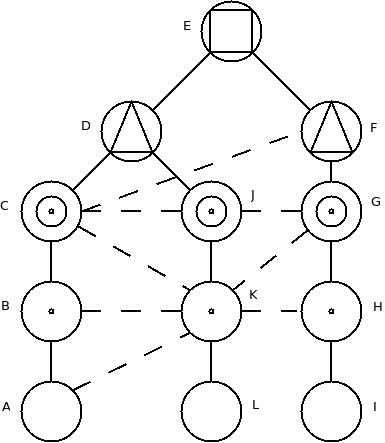
\includegraphics[width=0.5\textwidth]{Imagen/ejercicio9tema1.jpg}
\label{}
\end{figure}
\textbf{1.} Indique las rutas entre las siguientes centrales:\\
\begin{center}
\begin{tabular}{c c c c}
A$\to$L & AKL  		& L$\to$A 	& LKA 	\\
 		& ABKL		&			& LKJCBA	\\
 		& ABCKL		&			& LKJDCBA	\\
 		& ABCDJKL	&			& 	\\
A$\to$I & ABCFGHI  	& L$\to$I 	& LKHI 	\\
 		& ABCDEFGHI	&			& LKJGHI	\\
 		& 			&			& LKJDEFGHI	\\
I$\to$L & IHKL  	& 		 	&  	\\
 		& IHGKL		&			& 	\\
 		& IHGFEDJKL	&			& 	\\
\end{tabular}
\end{center}
\textbf{2.} Calcule el tráfico ofrecido y el tráfico cursado en la sección directa JC/CJ y en la sección final CD/DC.\\
\begin{center}
\begin{tabular}{| c | c | c | c | c | c | c | c | c | c | c | c | c |}
\hline
   & A & B  & C  & D  & E  & F  & G & H  & I  & J  & K  & L \\\hline
 A & - & 15 & 15 & 10 & 5  & 5  & 5 & 10 & 2  & 1  & 8  & 2 \\\hline
 B &   & -  & 15 & 10 & 4  & 5  & 5 & 10 & 2  & 1  & 9  & 1 \\\hline
 C &   &    & -  & 10 & 10 & 20 & 5 & 10 & 5  & 1  & 5  & 5 \\\hline
 D &   &    &    & -  & 10 & 10 & 5 & 1  & 1  & 1  & 0  & 1 \\\hline
 E &   &    &    &    & -  & 5  & 5 & 25 & 10 & 5  & 1  & 0 \\\hline
 F &   &    &    &    &    & -  & 5 & 5  & 10 & 5  & 1  & 1 \\\hline
 G &   &    &    &    &    &    & - & 10 & 5  & 10 & 5  & 5 \\\hline
 H &   &    &    &    &    &    &   & -  & 10 & 15 & 5  & 5 \\\hline
 I &   &    &    &    &    &    &   &    & -  & 10 & 5  & 5 \\\hline
 J &   &    &    &    &    &    &   &    &    & -  & 10 & 10 \\\hline
 K &   &    &    &    &    &    &   &    &    &    & -  & 10 \\\hline
\end{tabular}
\end{center}
Empezamos por calcular el tráfico ofrecido en un sentido y luego en el otro.
\begin{gather*}
TO_{CJ}=TO_{CJpropio}+TO_{AJ}+TO_{BJ}=3E\\
TO_{JC}=TO_{JCpropio}+TO_{KCdesb}+TO_{KBdesb}+TO_{KAdesb}+TO_{JA}+TO_{JB}\\
TO_{KC}=TO_{KCpropio}+TO_{LC}=10\\
TO_{KB}=TO_{KBpropio}+TO_{LB}=10\\
TO_{KA}=TO_{KApropio}+TO_{LA}=10\\
TO_{JC}=1+1+1+1+1+1=6\\
TO_{CD}=TO_{CDpropio}+TO_{CFdesb}+TO_{CJdesb}+TO_{CKdesb}+TO_{CE}+TO_{AD}+TO_{AE}+TO_{BD}+TO_{BE}\\
TO_{CF}=TO_{CFpropio}+TO_{CG}+TO_{CH}+TO_{CI}+TO_{BF}+TO_{BG}+TO_{BH}+TO_{BI}+TO_{AF}+TO_{AG}+\\
+TO_{AH}+TO_{AI}=84E\\
TO_{CJ}=3E\\
TO_{CK}=TO_{CKpropio}+TO_{BKdesb}+TO_{CL}\\
TO_{BK}=TO_{BKpropio}+TO_{AKdesb}+TO_{BL}\\
TO_{AK}=TO_{AKpropio}+TO_{AL}=10E\\
TO_{BK}=11E\\
TO_{CK}=11.1E\\
TO_{CD}=10+8.4+0.3+1.11+10+10+5+10+4=58.81E\\
TO_{DC}=TO_{DCpropio}+TO_{FCdesb}+TO_{JCdesb}+TO_{EC}+TO_{DB}+TO_{EB}+TO_{DA}+TO_{EA}\\
TO_{FC}=TO_{FCpropio}+TO_{GC}+TO_{HC}+TO_{IC}+TO_{FB}+TO_{GB}+TO_{HB}+TO_{IB}+TO_{FA}+TO_{GA}+\\
+TO_{HA}+TO_{IA}=84E\\
TO_{JC}=6E\\
TO_{DC}=10+8.4+0.6+10+10+5+10+4=58E
\end{gather*}
Para terminar calcularemos el tráfico cursado en cada uno de los tramos como $TC=TO(1-P_B)$ siendo $P_B$ la probabilidad de bloqueo en las rutas finales y la probabilidad de desbordamiento en las secciones directas.
\begin{gather*}
TC_{CJ}=TO_{CJ}(1-P_D)=2.7E\\
TC_{JC}=TO_{JC}(1-P_D)=5.4E\\
TC_{CD}=TO_{CD}(1-P_B)=58.22E\\
TC_{DC}=TO_{DC}(1-P_B)=57.42E
\end{gather*}
\end{exercise}
\begin{exercise}[10]
Utilice la red de la figura y la tabla adjunta (que es simétrica) para contestar a las siguientes preguntas:\\
NOTA: La probabilidad de pérdidas en ruta final es del 1 \% y la probabilidad de desbordamiento en secciones directas es del 10\% .
\begin{figure}[H]
\centering
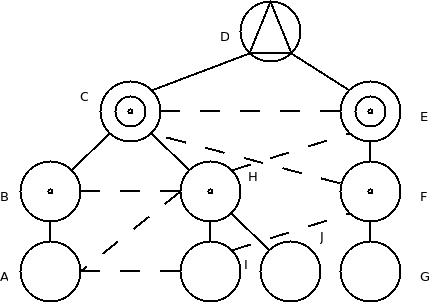
\includegraphics[width=0.5\textwidth]{Imagen/ejercicio10tema1.jpg}
\label{}
\end{figure}
\begin{center}
\begin{tabular}{| c | c | c | c | c | c | c | c | c | c | c |}
\hline
   & A & B  & C  & D  & E  & F  & G & H  & I  & J  \\\hline
 A & - & 15 & 15 & 10 & 3  & 5  & 4 & 10 & 5  & 1  \\\hline
 B &   & -  & 15 & 10 & 3  & 5  & 5 & 10 & 5  & 1  \\\hline
 C &   &    & -  & 10 & 20 & 30 & 1 & 1  & 5  & 2  \\\hline
 D &   &    &    & -  & 10 & 10 & 5 & 1  & 2  & 1  \\\hline
 E &   &    &    &    & -  & 5  & 5 & 25 & 10 & 5  \\\hline
 F &   &    &    &    &    & -  & 5 & 5  & 10 & 2  \\\hline
 G &   &    &    &    &    &    & - & 10 & 5  & 2  \\\hline
 H &   &    &    &    &    &    &   & -  & 5  & 2  \\\hline
 I &   &    &    &    &    &    &   &    & -  & 2  \\\hline
\end{tabular}
\end{center}
\textbf{1.} Rutas entre las siguientes centrales: A$\to$I, I$\to$G, A$\to$G, J$\to$G.\\
\begin{center}
\begin{tabular}{c c c c}
A$\to$I & AI  		& I$\to$G 	& IFG 		\\
 		& ABHI		&			& IHEFG		\\
 		& ABCHI		&			& IHCFG		\\
 		& 			&			& IHCDEFG	\\
A$\to$G & ABCFG  	& J$\to$G 	& JHEFG 	\\
 		& ABCDEFG	&			& JHCFG		\\
 		& 			&			& JHCDEFG	\\
\end{tabular}
\end{center}
\textbf{2.} Tráfico ofrecido y cursado en la sección directa CE/EC.\\
\begin{gather*}
TO_{CE}=TO_{CEpropio}+TO_{HEdesb}+TO_{BE}+TO_{AE}\\
TO_{HE}=TO_{HEpropio}+TO_{IFdesb}+TO_{HF}+TO_{HG}+TO_{JE}+TO_{JF}+TO_{JG}\\
TO_{IF}=TO_{IFpropio}+TO_{IG}=15E\\
TO_{HE}=50.5E\\
TO_{CE}=31.05E\\
TC_{CE}=TO_{CE}(1-P_B)=30.7395E\\
TO_{EC}=TO_{ECpropio}+TO_{FC'desb}+TO_{EB}+TO_{EA}\\
TO_{FC'}=TO_{FCpropio}+TO_{FB}+TO_{FA}+TO_{GC}+TO_{GB}+TO_{GA}=50E\\
TO_{EC}=31E\\
TC_{EC}=30.69E
\end{gather*}
\end{exercise}
\begin{exercise}[11]
En la comunidad Autónoma de Andalucía (con 8 provincia), existe una central secundaria en cada provincia para cursar el tráfico provincial, y solo una central terciaria situada en Sevilla para cursar el tráfico interprovincial. Ahí es precisamente donde se sitúa el proveedor de servicios de Internet o ISP. Asumamos que cada provincia está compuesta por 10 localidades (es un escenario ficticio pero es para poder simplificar el ejercicio), y en cada una de ellas se encuentra situada una central primaria, para cursar el tráfico local. Asimismo, cada localidad está formada por una serie de barrios, y en cada uno de ellos existe una central local con capacidad para 2000 líneas.\\
La arquitectura de la red es la siguiente. Todas las centrales locales bajo la misma central primaria se encuentran conectadas mediante enlaces directos para cursar, en primera instancia, el tráfico local. La probabilidad de desbordamiento en estas secciones directas es del 10\% . Además, cada central local se encuentra conectada a la central secundaria de la que depende jerárquicamente mediante secciones directas con probabilidad probabilidad de desbordamiento del 15\%, para cursar,en primera instancia, todo el tráfico provincial e interprovincial. Cada central local se conecta por sección final a su central primaria. A su vez, cada central primaria se conecta mediante sección final a su central secundaria y cada central secundaria se conecta, por sección final a su central terciaria, formando de esta forma la ruta final, cuya probabilidad de bloqueo es del 1\%(asuma que si se bloquea una llamada, se bloquea en la última de las secciones). Considere también despreciable el tráfico local entre abonados de la misma central local.\\
Se ofrece una tarifa plana entre las 18:00 y las 8:00 de la mañana, para aprovechar el periodo donde menos tráfico vocal se cursa.\\
Se ha medido el siguiente tráfico por ususario en este escenario:
\begin{itemize}
\item 2 llamadas locales en la hora cargada, de 144 segundos de duración.
\item 1 llamada provincial o interprovincial en la hora cargada de 450 segundos de duración.
\item La distribución entre llamadas provinciales e interprovinciales es de 30\% y 70\%, respectivamente.
\item 1 llamada de datos de 42 minutos de duración.
\end{itemize}
\textbf{NOTA:} Para los apartados 3 y 4 (y solo para ellos) utilize las siguientes aproximaciones de la Erlang-B: $B(c,A_o)=0.01=\sfrac{A_o}{85c}$; $B(c,A_o)=0.1=\sfrac{A_o}{102c}$ y para la Erlang-C: $C(c,A_o)=0.01=\sfrac{7A_o}{c}$; $C(c,A_o)=0.1=\sfrac{53A_o}{c}$.\\
Se le pide que dimensione alguno de los enlaces de la red anterior:\\
\textbf{1.} Calcule el número de sistemas MIC de norma Europea en el enlace entre la central local y la central primaria.\\
\textbf{2.} Calcule el número de barrios por localidad sabiendo que la capacidad de la central primaria es 1090E\\
\textbf{3.} ¿Cuántos canales duplex serían necesarios para conectar la central primaria y su secundaria jerarquica?\\
\textbf{4.} El enlace entre las centrales secundarias y su terciaria se realiza mediante SDH. Calcule la jerarquía mínima SDH  necesaria para cursar todo el tráfico.\\
\textbf{5.} ¿Se podría utilizar SNCP en el enlace anterior? Razone su respuesta.
\end{exercise}